%**************************************************************************************
% License:
% CC BY-NC-SA 4.0 (http://creativecommons.org/licenses/by-nc-sa/4.0/)
%**************************************************************************************

\documentclass[notes]{beamer}

\mode<presentation> {

\usetheme{Madrid}

% Burnt orange
\definecolor{burntorange}{rgb}{0.8, 0.33, 0.0}
\colorlet{beamer@blendedblue}{burntorange}
% Pale yellow
\definecolor{paleyellow}{rgb}{1.0, 1.0, 0.953}
\setbeamercolor{background canvas}{bg=paleyellow}
% Secondary and tertiary palett
\setbeamercolor*{palette secondary}{use=structure,fg=white,bg=burntorange!80!black}
\setbeamercolor*{palette tertiary}{use=structure,fg=white,bg=burntorange!60!black}

% To remove the footer line in all slides uncomment this line
%\setbeamertemplate{footline}
% To replace the footer line in all slides with a simple slide count uncomment this line
%\setbeamertemplate{footline}[page number]

% To remove the navigation symbols from the bottom of all slides uncomment this line
%\setbeamertemplate{navigation symbols}{}
}

\usepackage{amsmath}
\usepackage{bm}
\usepackage{breqn}
\usepackage{cancel}
\usepackage{graphicx} % for figures
\usepackage{subcaption} % for subplots 
\usepackage[labelsep=space,tableposition=top]{caption}
\renewcommand{\figurename}{Fig.} 
\usepackage{cleveref}
\usepackage{caption,subcaption}% http://ctan.org/pkg/{caption,subcaption}
\usepackage{booktabs} % Allows the use of \toprule, \midrule and \bottomrule in tables
\usepackage{multirow}
\usepackage{tabularx}
\usepackage{siunitx}
\usepackage{cleveref}
\usepackage{xcolor}

% To print 2 slides on a page
%\usepackage{handoutWithNotes}
%\pgfpagesuselayout{2 on 1}[border shrink=2mm]
%----------------------------------------------------------------------------------------
%	TITLE PAGE
%----------------------------------------------------------------------------------------
% The short title appears at the bottom of every slide, the full title is only on the title page
\title[CE394M: intro to plasticity]{CE394M: An introduction to plasticity} 
\author{Krishna Kumar} % name
\institute[UT Austin] % institution 
{
University of Texas at Austin \\
\medskip
\textit{
  \url{krishnak@utexas.edu}} % Your email address
}
\date{\today} % Date, can be changed to a custom date

\begin{document}

\begin{frame}
\titlepage % title page as the first slide
\end{frame}

\begin{frame}
 % Table of contents slide, comment this block out to remove it
 \frametitle{Overview}
  %Throughout your presentation, if you choose to use \section{} and \subsection{} 
  %commands, these %will automatically be printed on this slide as an overview 
 \tableofcontents
\end{frame}

%----------------------------------------------------------------------------------------
% slides
%----------------------------------------------------------------------------------------
\section{Constitutive modeling}
%----------------------------------------------------------------------------------------
\begin{frame}
\frametitle{Constitutive law}
\mode<beamer>{
Constitutive law is the stress-strain relationship: $\sigma = f(\varepsilon) \rightarrow \sigma = \mathbf{D} \cdot \varepsilon$
}
\mode<handout>{
	\vspace{1.5cm}
}
\begin{figure}
	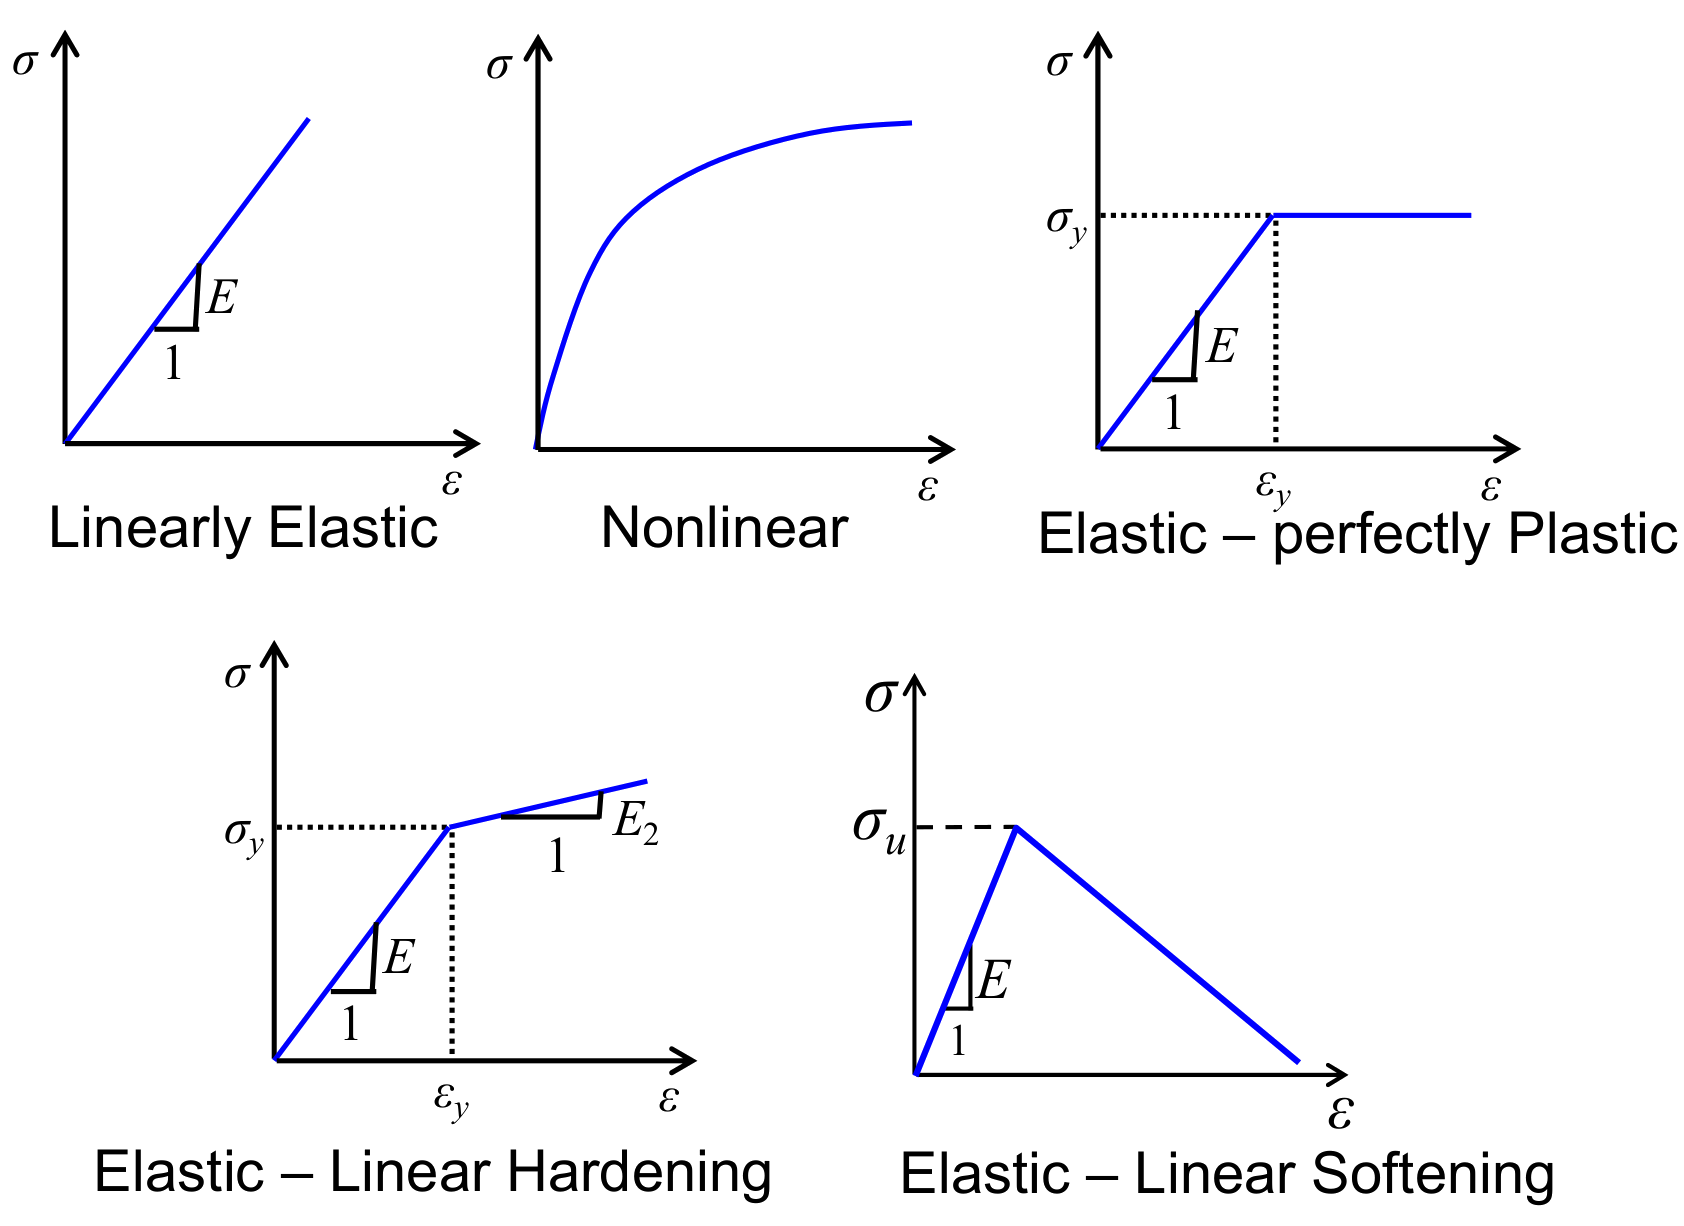
\includegraphics[width=0.75\textwidth]{figs/constitutive-law.png}
\end{figure}
\end{frame}

%----------------------------------------------------------------------------------------
\begin{frame}
\frametitle{Isotropic linear elasticity}
\mode<beamer>{
	$\sigma = \mathbf{D^{el}} \cdot \varepsilon$ where $\mathbf{D^{el}}$ is the elastic stiffness matrix.
}
\mode<handout>{
	\vspace{1.5cm}
}
\begin{figure}
	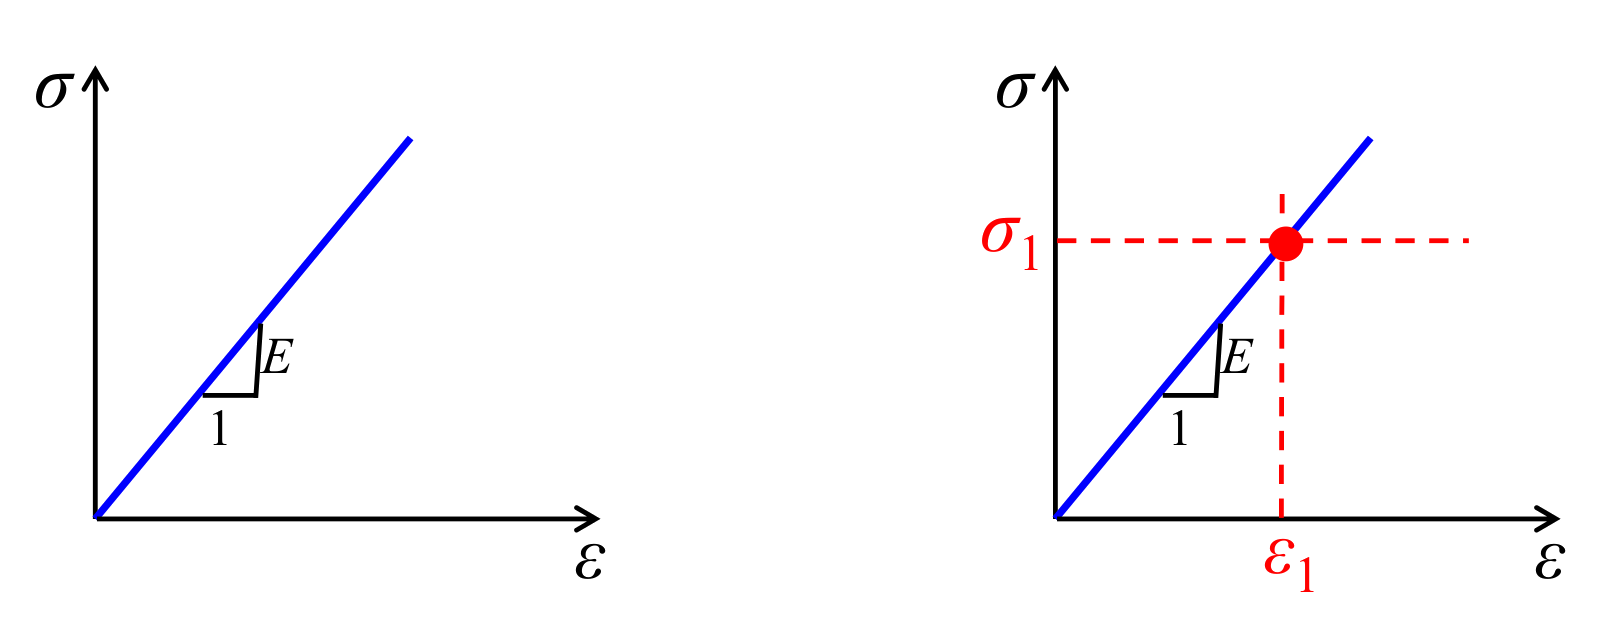
\includegraphics[width=\textwidth]{figs/linear-elasticity.png}
	\caption*{The knowledge of strain alone allows us to obtain the stress value.}
\end{figure}
\end{frame}

%----------------------------------------------------------------------------------------
\begin{frame}
\frametitle{Nonlinear elasticity}
\textbf{Hyperbolic model (Duncan and Chang., 1970)}
\mode<beamer>{
	\begin{align*}
	(\sigma_1 - \sigma_3) & = \frac{\varepsilon}{a + b \varepsilon} \\
	a & = \frac{1}{E_i} \quad b = \frac{1}{(\sigma_1 - \sigma_3)_{ult}}
	\end{align*}

}
\mode<handout>{
	\vspace{2cm}
}
\begin{figure}
	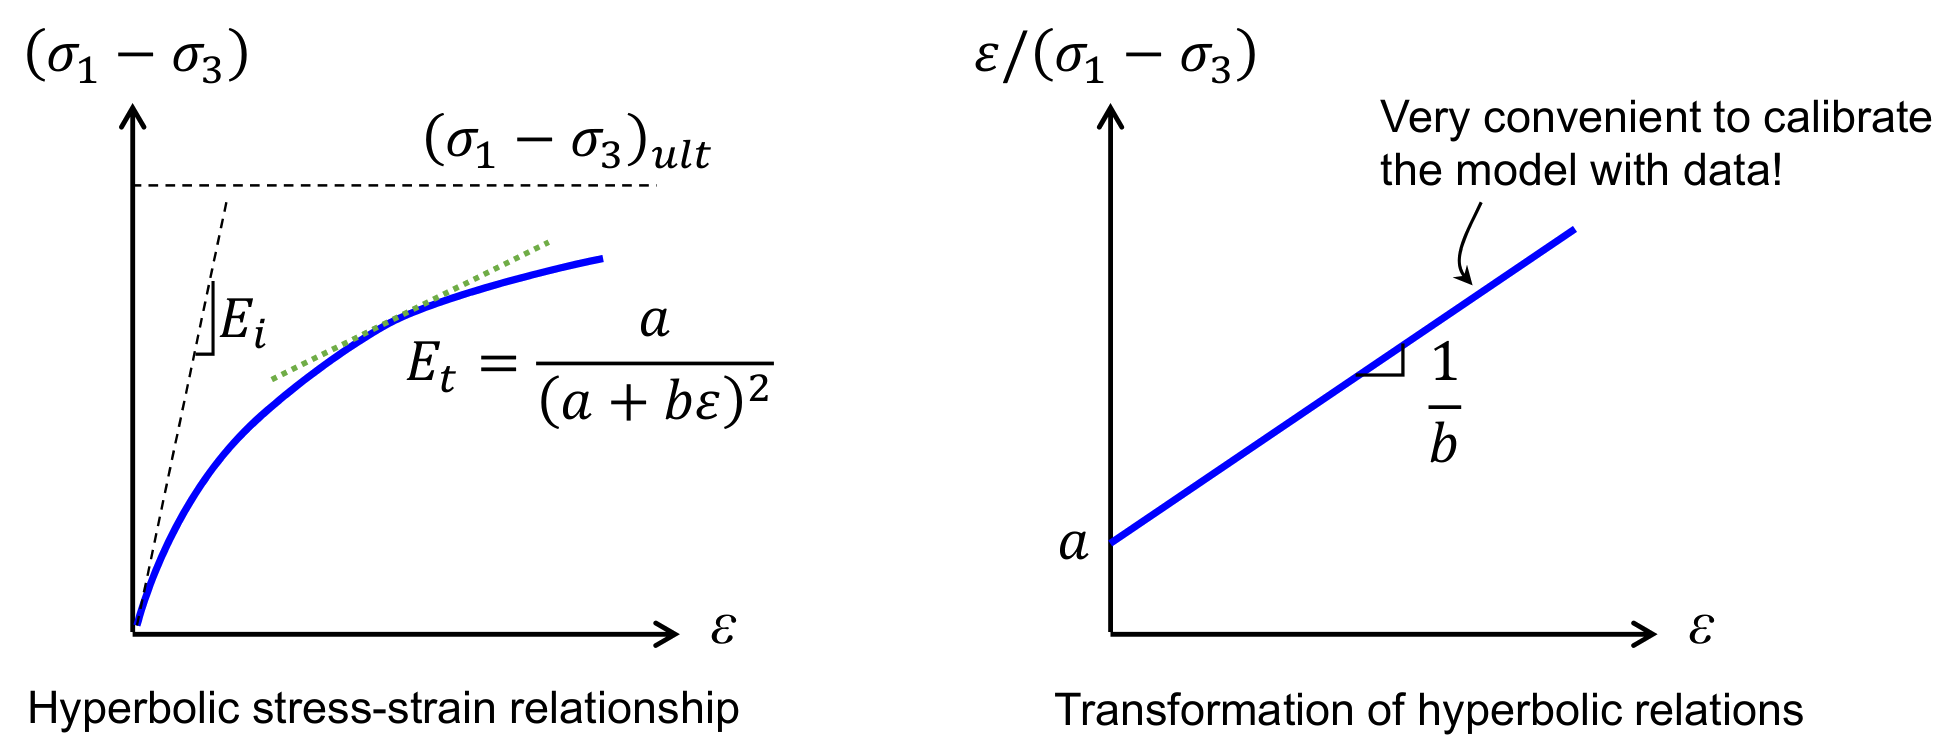
\includegraphics[width=0.8\textwidth]{figs/hyperbolic.png}
	\caption*{There is no physical meaning to $(\sigma_1 - \sigma_3)_{ult}$. The $(\sigma_1 - \sigma_3)_f$ is determined from the strength criteria $\tau = c + \sigma^\prime \tan \phi^\prime$ (drained) or $\tau = s_u$ (total stress undrained).}
\end{figure}
\end{frame}

%----------------------------------------------------------------------------------------
\section{Plasticity}

%----------------------------------------------------------------------------------------
\begin{frame}
\frametitle{Classical plasticity}
\begin{figure}
	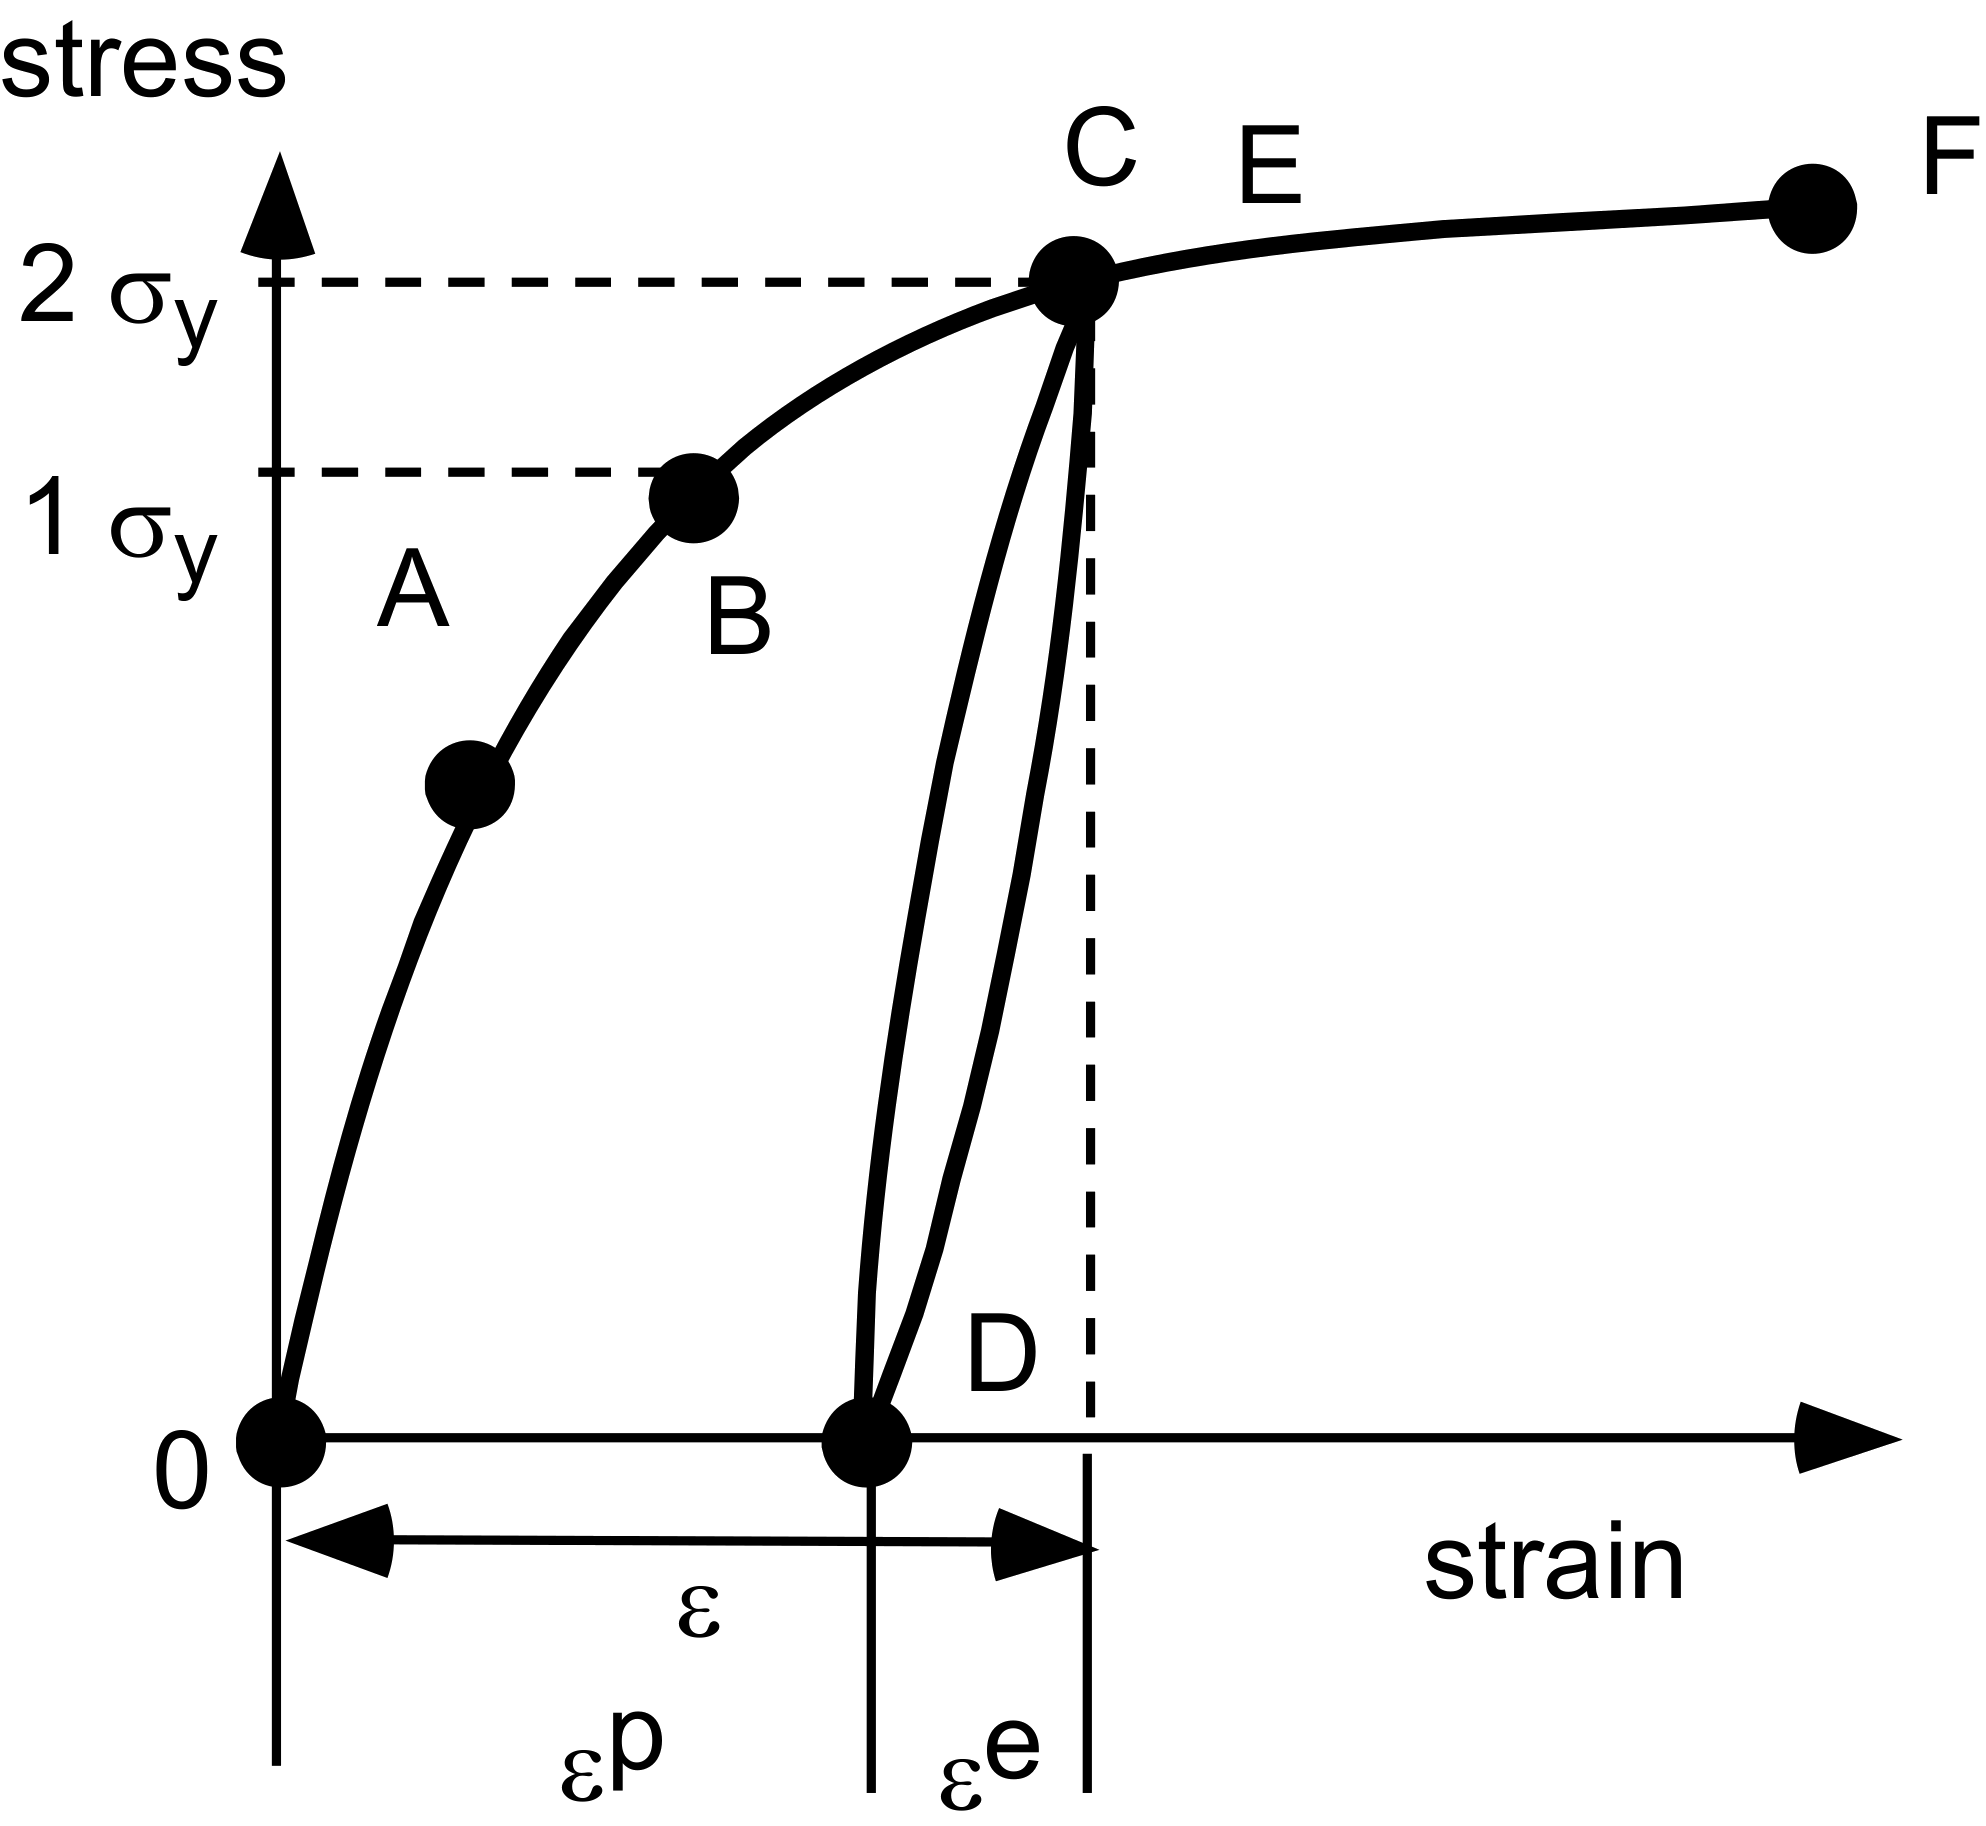
\includegraphics[width=0.6\textwidth]{figs/stress-strain-plasticity.png}
	\caption*{Specimen 1 at point 0 same as specimen 2 at point D, but yield stress of specimen 2 is greater than the yield stress of specimen 1 due to \textbf{plastic hardening}.}
\end{figure}
\end{frame}

\note{
Uniaxial tension test on metal bar:
\begin{table}
	\begin{tabular}{l l}
		\toprule
		 O$\rightarrow$A & Linear elastic, reversible \\
 		 A$\rightarrow$B & Nonlinear elastic, reversible \\
 		 B    & Starts to yield \\
 		 B$\rightarrow$C & Nonlinear elasto-plastic, irreversible \\
 		 C$\rightarrow$D & Elastic with hysteresis \\
 		 C$\rightarrow$F & Nonlinear elasto-plastic, irreversible \\
 		 F    & Peak stress at failure \\
 		 \bottomrule
	\end{tabular}
\end{table}
	$\varepsilon = \varepsilon^e + \varepsilon^p$, where $e$ is elastic and $p$ is plastic.
}


%----------------------------------------------------------------------------------------
\begin{frame}
\frametitle{Classical plasticity}
\mode<beamer>{
	\begin{itemize}
		\item \textbf{Plastic behavior}: The direction of plastic strains is governed by
		the current stress state $\sigma$. $d\sigma = f(d\varepsilon) \rightarrow d\sigma = \mathbf{D}^{e} \cdot d\varepsilon$. 
		\item \textbf{Elastic behavior}: The direction of elastic strains is governed by
		the stress state increment $\delta \sigma$ direction.
		\item \textbf{Plastic models}
		\begin{itemize}
			\item Rigid - perfectly plastic model - used in static limit equilibrium analysis (no elastic strain and no strain hardening / softening)
			\item Linear elastic - perfectly plastic model (Drucker-Prager and Mohr Coulomb
			models)
			\item Hybrid model (nonlinear elastic with perfectly plastic - Duncan and Chang)
			\item Work (or strain) hardening plasticity model (Cam-Clay model)
		\end{itemize}
	\end{itemize}
	
}
\mode<handout>{
	\vspace{4cm}
}
\begin{figure}
	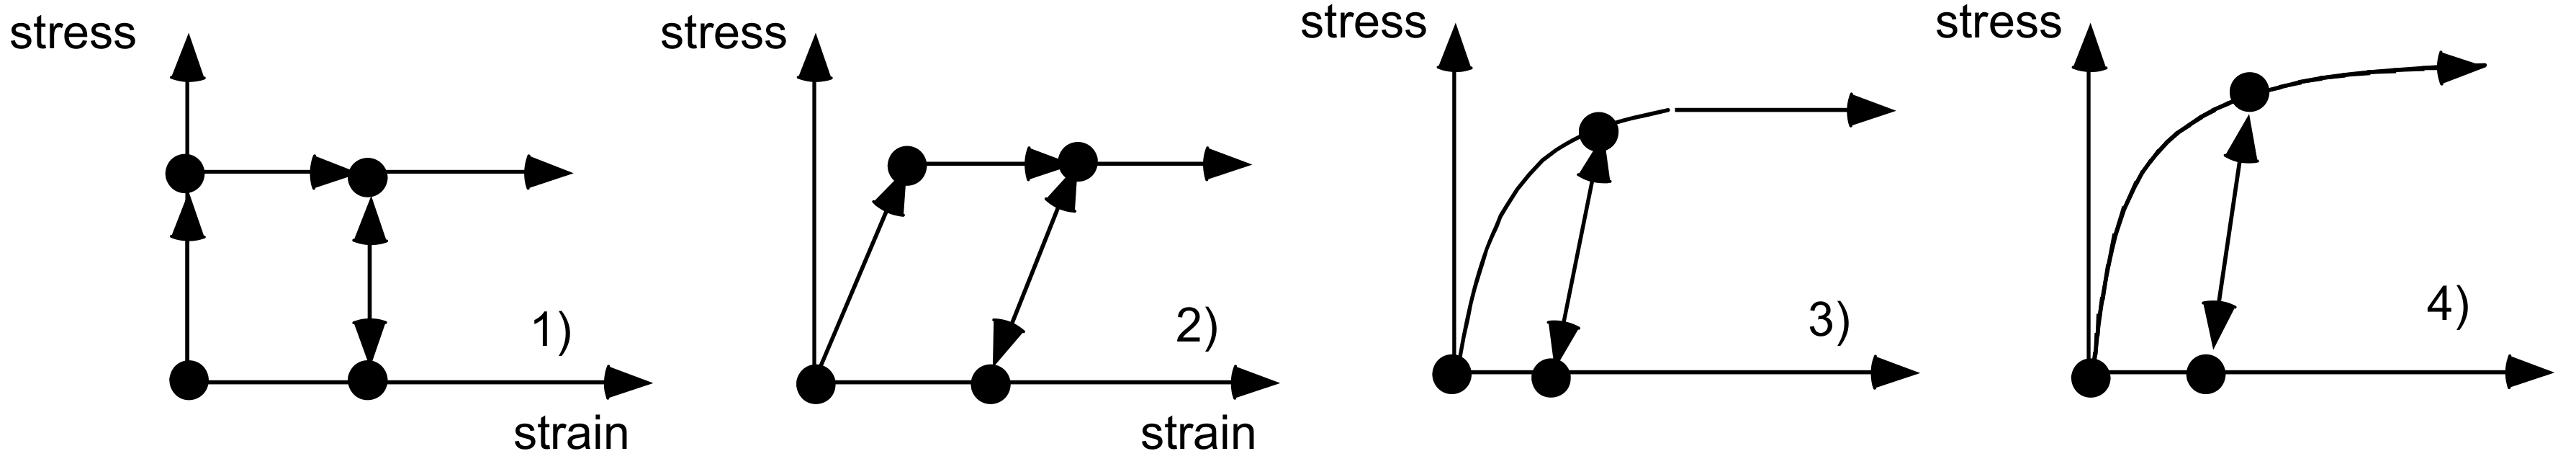
\includegraphics[width=0.9\textwidth]{figs/classical-plasticity.png}
\end{figure}
\end{frame}

%----------------------------------------------------------------------------------------
\begin{frame}
\frametitle{Elasto-plastic materials}
\mode<beamer>{
Main distinctive feature of elasto-plastic materials:
``\textit{irreversibility}'' $\rightarrow$ \textbf{Plastic deformation } $\varepsilon^p$	
}
\mode<handout>{
	\vspace{1cm}
}
\begin{figure}
	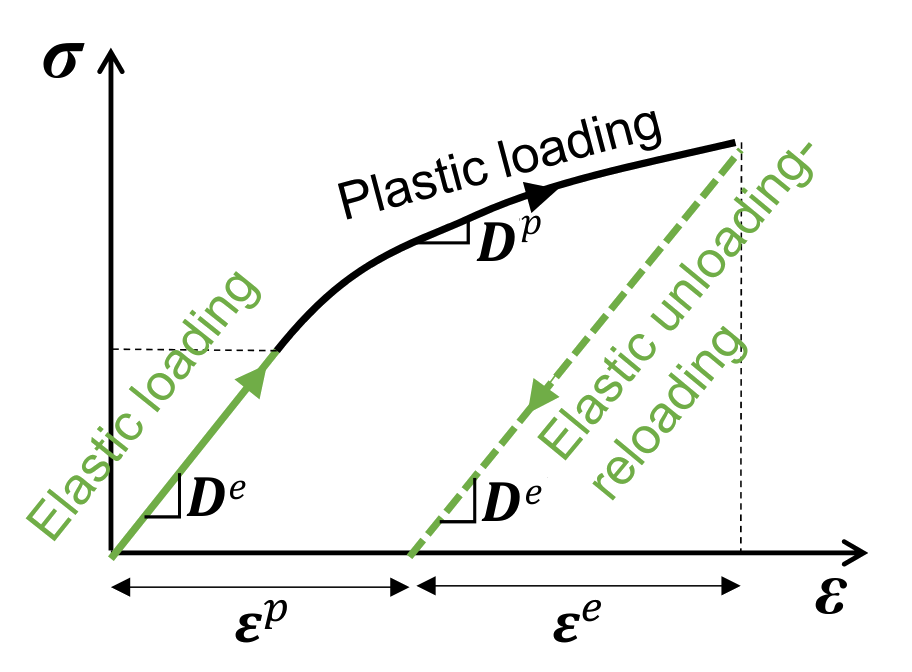
\includegraphics[width=0.6\textwidth]{figs/elasto-plastic.png}
\end{figure}
\mode<beamer>{
	\begin{equation*}
	\varepsilon = \varepsilon^e + \varepsilon^p \quad d\varepsilon = d\varepsilon^e + d\varepsilon^p
	\end{equation*}
}
\mode<handout>{
	\vspace{1cm}
}
\end{frame}

%----------------------------------------------------------------------------------------
\begin{frame}
\frametitle{Basic concepts of classical plasticity}
To formulate an elasto‐plastic constitutive model we need:
\mode<beamer>{
	\begin{enumerate}
		\item \textbf{Elastic stress-strain relationship:} $\sigma = \mathbf{D}^e \varepsilon^e = \mathbf{D}^e (\varepsilon - \varepsilon^p)$. Describe elastic response.

		\item  \textbf{Yield function}: defines the condition for the onset of plastic strain. Depends on the stress state $\sigma$ and state parameters (e.g., in MC they are cohesion and friction angle). $F(\sigma^\prime, Wp) = 0$.

		\item \textbf{Plastic potential ($G(\sigma, Wp) = 0$)} defines the direction of plastic strains. Depends on stress state $\sigma$ and state parameter (for e.g., is dilatancy in MC). Note that the direction of $d\varepsilon^p$ doesn't depend on $d\sigma$ but on the actual stress state $\sigma$. \textbf{Flow rule} $\varepsilon^p = \lambda (dG/d\sigma)$.
		
		\item \textbf{Hardening rule / Hardening law (h)} defines how $F$ changes with plastic strains. Yield function $F = f(\text{stress state}, W_p)$, where $W_p$ is a function of plastic strains. Describes the evolution of state parameters depending on the plastic strain $\varepsilon^p$.
		
	\end{enumerate}
}
\mode<handout>{
	\vspace{6cm}
}
\end{frame}


%----------------------------------------------------------------------------------------
\begin{frame}
\frametitle{Yield functions}
defines when plastic strains occur. If the material is
isotropic, we can use the principal stresses to define the stress state.
\begin{figure}
	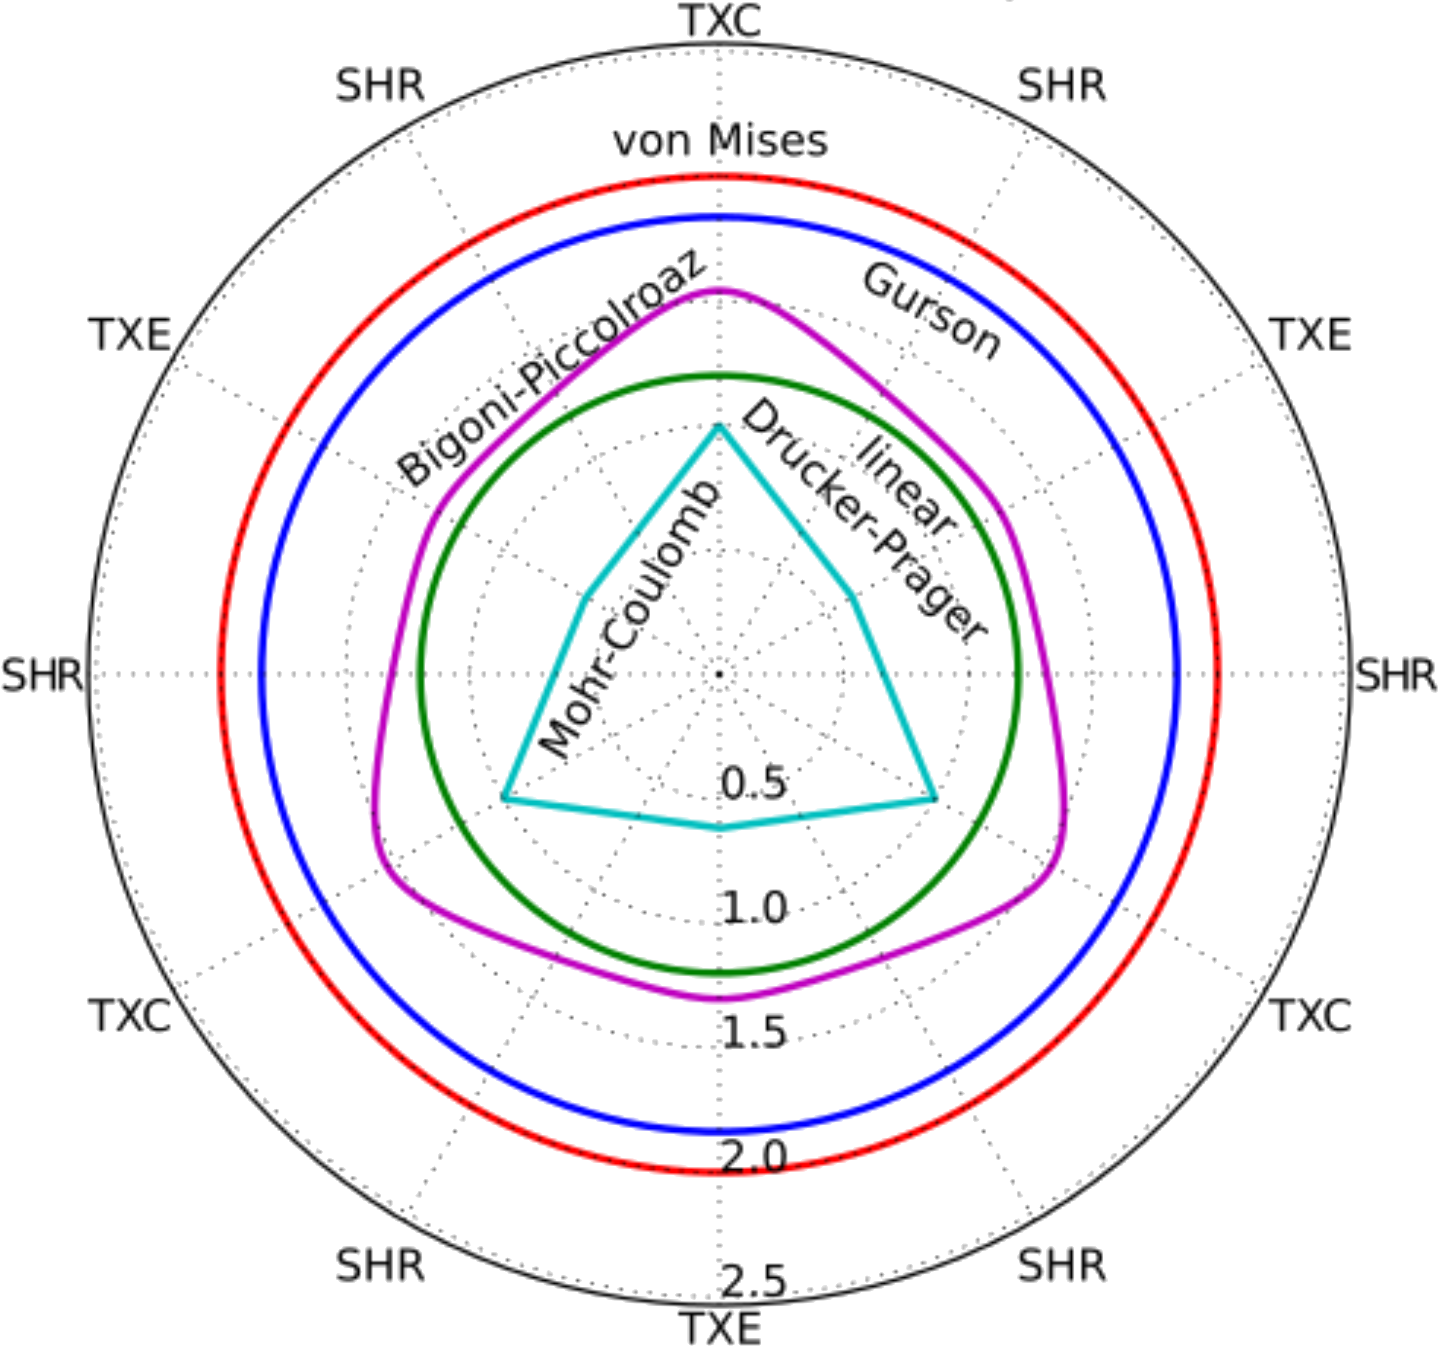
\includegraphics[width=0.55\textwidth]{figs/octahedral-stress-profile.png}
	\caption*{Wikipedia}
\end{figure}
\end{frame}

\note{
	Yield function $F(\sigma, Wp) = 0$.
	\begin{itemize}
		\item if $F = 0$ under loading: yielding and plastic strains and in unloading: elastic strains.
		\item if $F < 0$ elastic domain.
		\item if $F > 0$ impossible.
	\end{itemize}
	\begin{figure}
		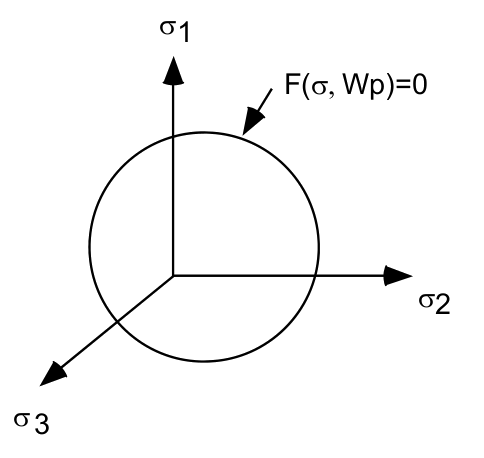
\includegraphics[width=0.4\textwidth]{figs/yieldfn.png}
	\end{figure}


}

%----------------------------------------------------------------------------------------
\begin{frame}
\frametitle{Hardening law}
How the threshold of yielding changes with plastic strain or how the yield function changes with plastic strain.
\begin{figure}
	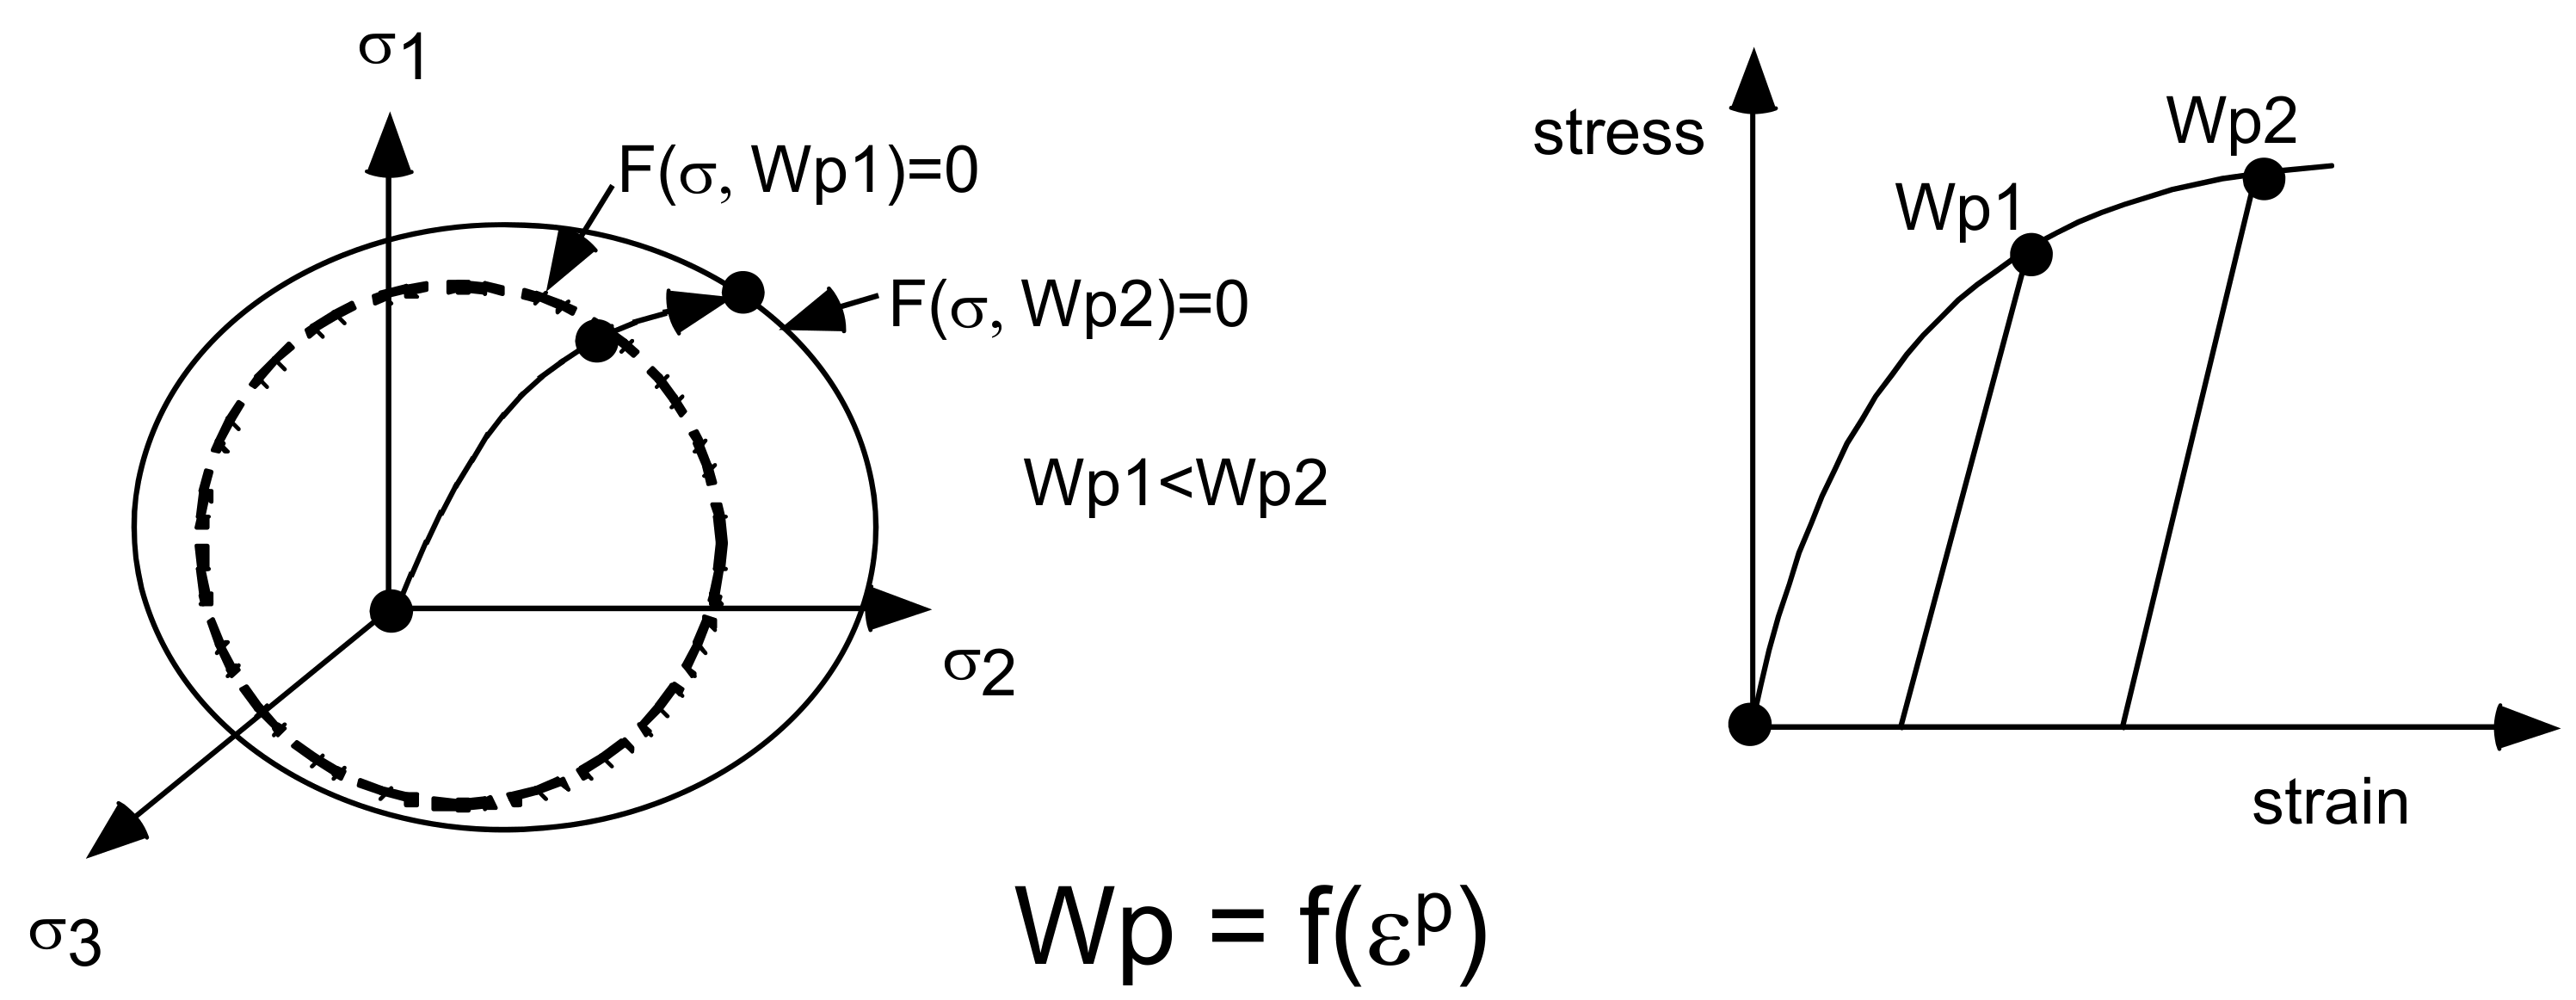
\includegraphics[width=0.85\textwidth]{figs/hardening-law.png}
\end{figure}
\end{frame}

\subsection{Equations of plasticity}

%----------------------------------------------------------------------------------------
\begin{frame}
\frametitle{Equations of elasto-plasticity: 1. Stress-strain relation}
\mode<beamer>{
	Describes the incremental stress-strain relationship. 
	\begin{equation*}
	d\sigma = D^e \cdot d\varepsilon^e = D^e \cdot (d\varepsilon - d\varepsilon^p)
	\end{equation*}
	Where $D^e$ is the elastic stiffness matrix. $^e$ denotes the elastic part.
}
\mode<handout>{
	\vspace{2cm}
}
\begin{figure}
	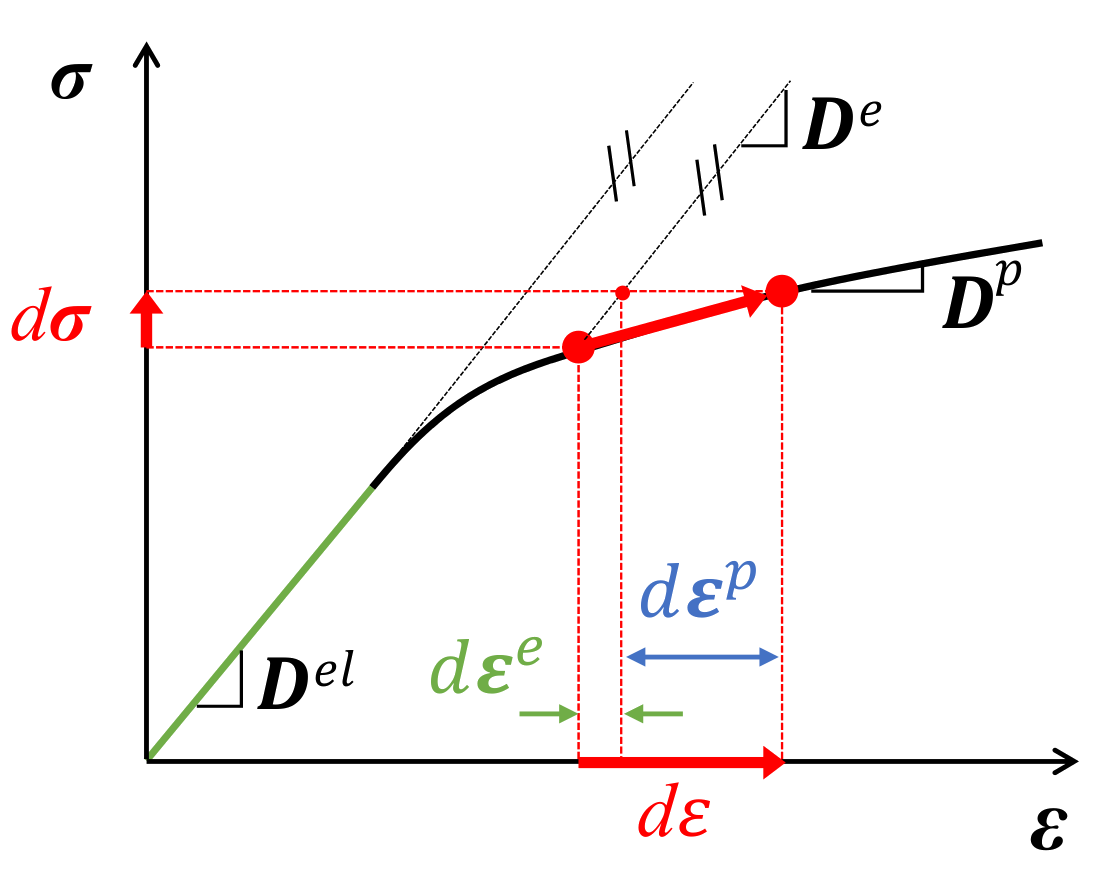
\includegraphics[width=0.6\textwidth]{figs/stress-strain.png}
\end{figure}
\end{frame}

%----------------------------------------------------------------------------------------
\begin{frame}
\frametitle{Equations of elasto-plasticity: 2. Flow rule}
\mode<beamer>{
	\begin{itemize}
		\item Specifies the direction of plastic strain increments at every yield stress state. It is very important because it controls the ratio of the volumetric and deviatoric components (e.g., dilatancy of the material). 
		
		\item States that the plastic strain increments ($d\varepsilon^p$) are normal to the plastic potential surface ($G$). 
		\begin{equation*}
		d\varepsilon^p =  d\lambda \cdot \vec{P}
		\end{equation*}
		
		Note: typically $\vec{P}$ is \textbf{not} a  unit vector, so $\vec{P}$ also controls the magnitude of $d \vec{\varepsilon_p}$ (in addition to the direction).
		
		\item In many cases, $\vec{P}$ is chosen as the gradient of a function $g$ (if it exists) such that:
		
		\begin{equation*}
		\vec{P} = \frac{\partial G}{\partial \sigma}
		\end{equation*}
	\end{itemize}		
}
\mode<handout>{
	\vspace{2cm}
}
\end{frame}

%----------------------------------------------------------------------------------------
\begin{frame}
\frametitle{Equations of elasto-plasticity: 3. Consistency condition}
\mode<beamer>{
	States that the elastic limit is defined by the yield surface, enforcing points in plastic condition to \textbf{remain} on the yield surface.
	\begin{equation*}
		dF = \left(\frac{\partial F}{\partial \sigma}\right)^T \cdot d \sigma + \frac{\partial F}{\partial Wp}\cdot dWp = 0
	\end{equation*}
	Where $D^e$ is the elastic stiffness matrix. $^e$ denotes the elastic part.
	
	E.g., strain hardening in tension for steel.
}
\mode<handout>{
	\vspace{2cm}
}
\begin{figure}
	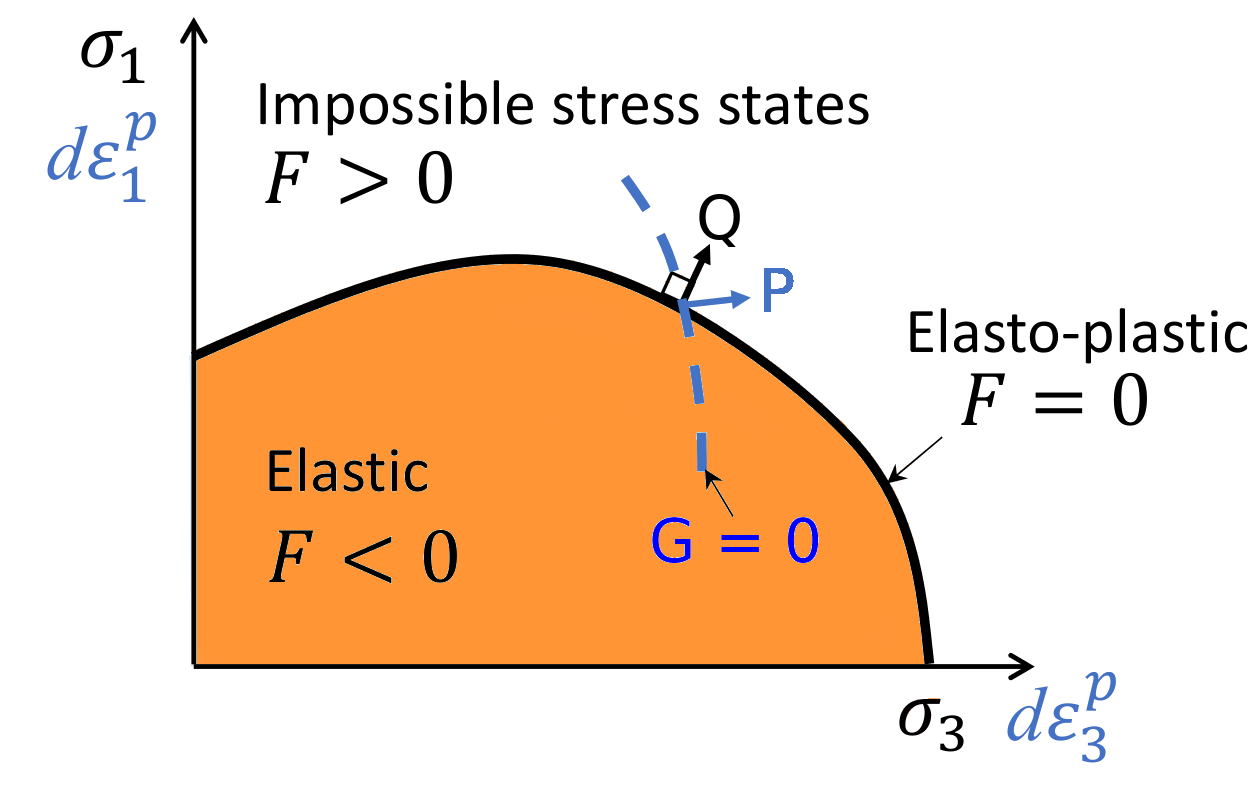
\includegraphics[width=0.6\textwidth]{figs/yield.png}
\end{figure}
\end{frame}

\note {
	\begin{align*}
	n &= \frac{\partial F}{\partial \sigma} \\
	m &= \frac{\partial G}{\partial \sigma}
	\end{align*}
}


%----------------------------------------------------------------------------------------
\begin{frame}
\frametitle{Drucker's postulate}

Drucker (1952) established that for a stable inelastic material in a closed stress cycle, a positive work must be done. 

\mode<beamer>{
	\begin{equation*}
		dW^p > 0 \rightarrow d\sigma \cdot d\varepsilon^p > 0
	\end{equation*}
	This requirement is satisfied if the normality condition is assumed (but is not the only solution). The gradient of the yield surface (i.e., normal to the surface)	
	\begin{equation*}
		\vec{Q} = \frac{\partial F}{\partial \sigma} = \vec{P}
	\end{equation*}
	It also imposes a constraint that the yield surface must be convex.
}
\mode<handout>{
	\vspace{3cm}
}
\begin{figure}
	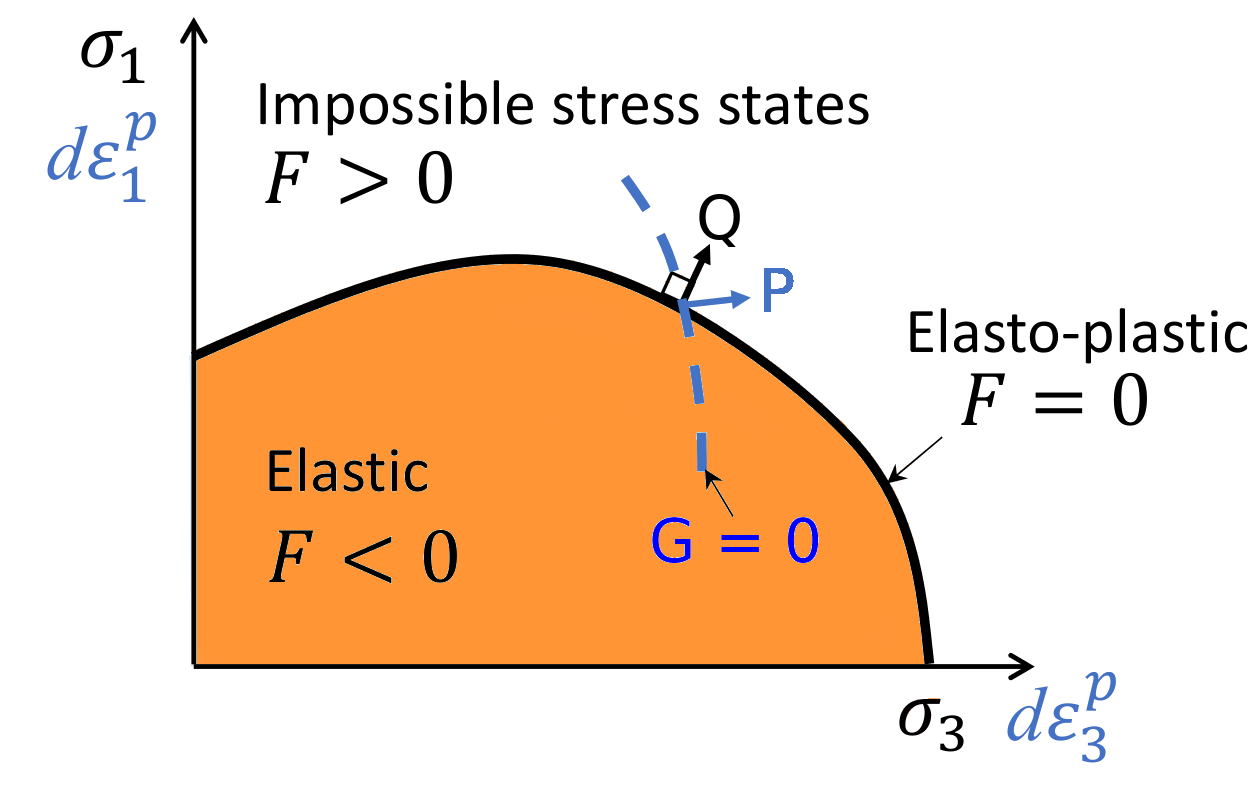
\includegraphics[width=0.4\textwidth]{figs/yield.png}
\end{figure}
\end{frame}

\note {
\begin{align*}
Q &= \frac{\partial F}{\partial \sigma} \\
P &= \frac{\partial G}{\partial \sigma}
\end{align*}
}



%----------------------------------------------------------------------------------------
\begin{frame}
\frametitle{Equations of elasto-plasticity: 3. Consistency condition}
The consistency condition can be written as:
	\begin{align*}
	dF & = \left(\frac{\partial F}{\partial \sigma}\right)^T \cdot d \sigma + \frac{\partial F}{\partial Wp}\cdot dWp & = 0 \\
	%
	 & = \left(\frac{\partial F}{\partial \sigma}\right)^T \cdot d \sigma + \frac{\partial F}{\partial Wp}\cdot \frac{\partial Wp}{\partial \varepsilon^p}\cdot d \varepsilon^p & = 0 \\
	% 	
	 & = \left(\frac{\partial F}{\partial \sigma}\right)^T \cdot d \sigma + \textcolor{orange}{\frac{\partial F}{\partial Wp}\frac{\partial Wp}{\partial \varepsilon^p}\cdot\frac{\partial G}{\partial 	\sigma}} d\lambda  & = 0 \\
	%
	dF & = \left(\frac{\partial F}{\partial \sigma}\right)^T \cdot d \sigma - \textcolor{orange}{H} d\lambda & = 0.
	\end{align*}

	if $\textcolor{orange}{H} > 0$: Hardening, if $\textcolor{orange}{H} = 0$: perfect plasticity, if $\textcolor{orange}{H} < 0$: softening.
\end{frame}


%----------------------------------------------------------------------------------------
\begin{frame}
\frametitle{Hardening v Softening}
Linear elastic – hardening plastic material  $\textcolor{orange}{H} > 0$
\begin{figure}
	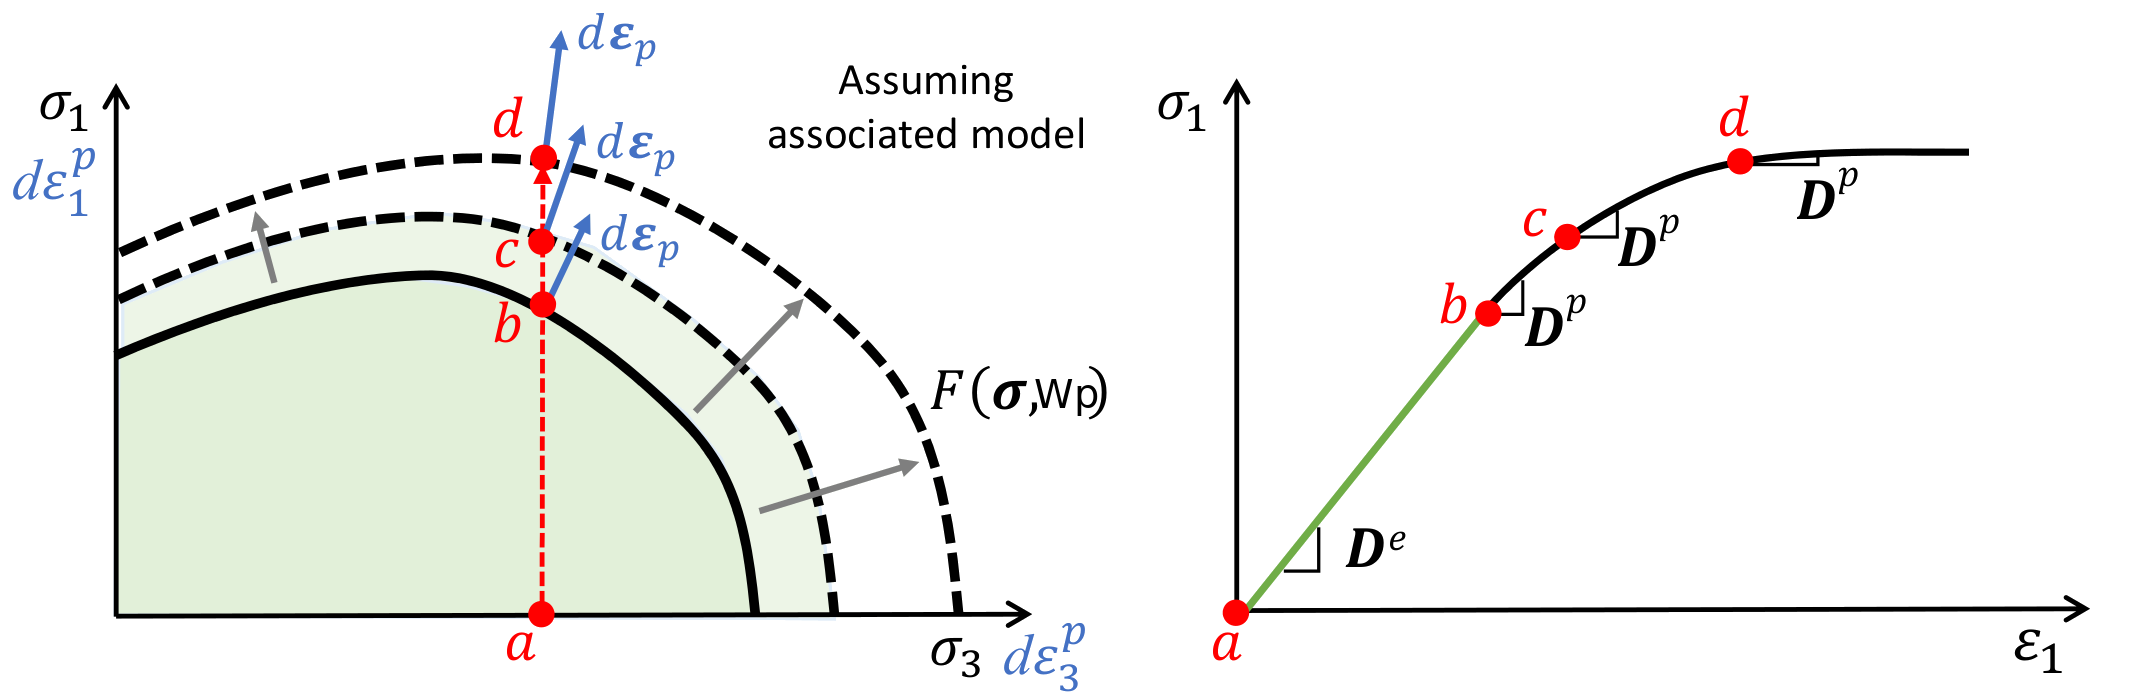
\includegraphics[width=0.8\textwidth]{figs/hardening-plastic.png}
\end{figure}
Linear elastic – softening plastic material  $\textcolor{orange}{H} < 0$
\begin{figure}
	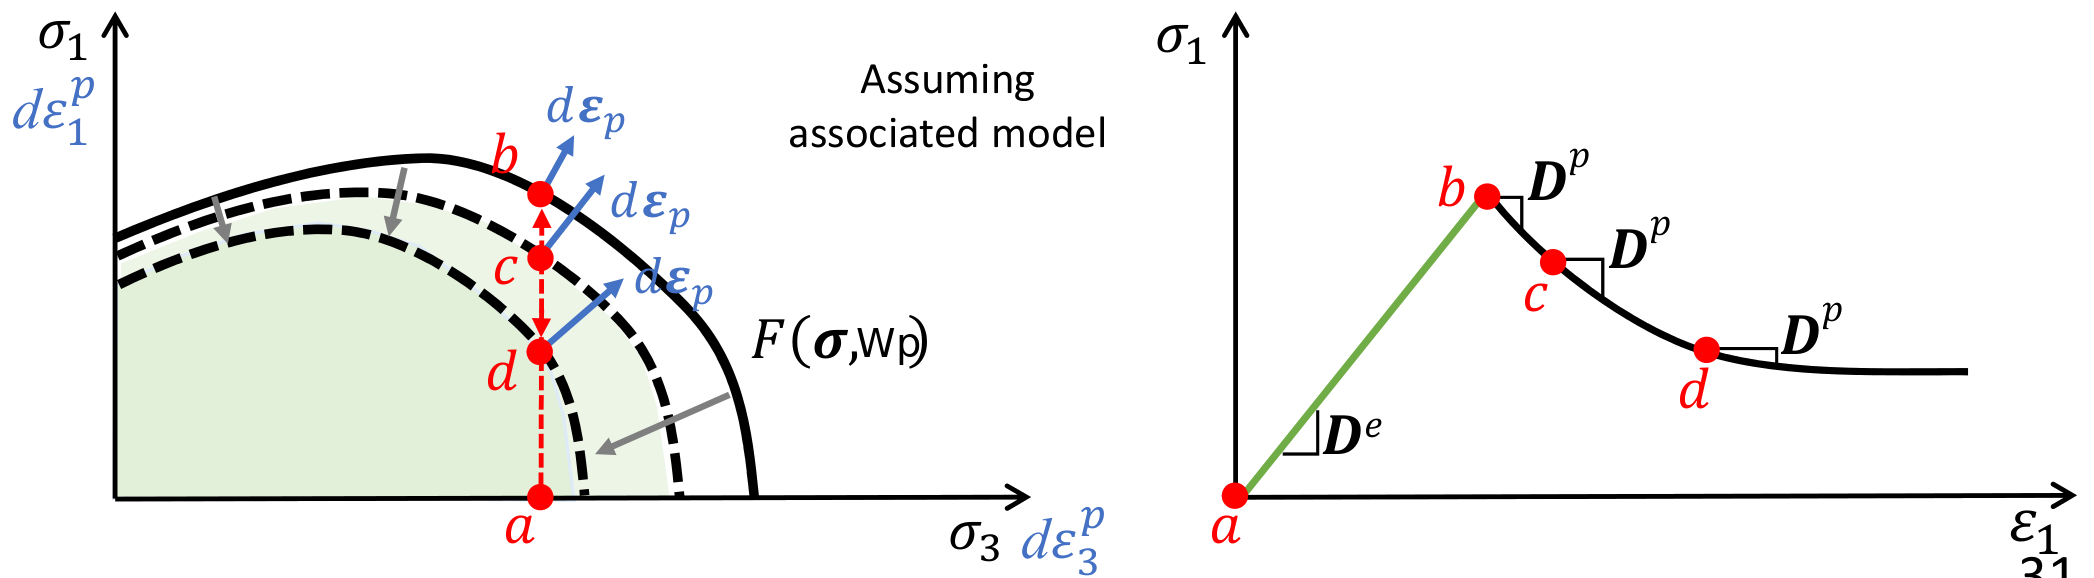
\includegraphics[width=0.8\textwidth]{figs/softening-plastic.png}
\end{figure}
\end{frame}

\end{document}
